\documentclass[tikz,border=3pt]{standalone}
\usepackage{tikz}
\usepackage{amsmath,amssymb}

\begin{document}
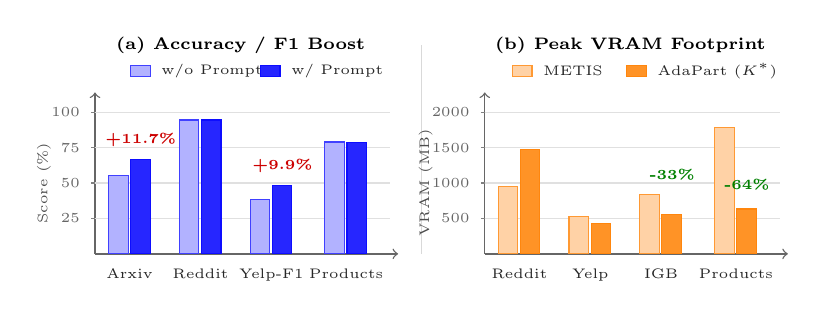
\begin{tikzpicture}[font=\sffamily]

% Total column width: 8.6cm (matches 0.98\columnwidth)

% =========================================================================
% Subfigure (a): Accuracy & F1 Boost
% =========================================================================
\begin{scope}[local bounding box=subfigA]
    % Title
    \node[font=\bfseries\fontsize{6.5}{7.5}\selectfont] at (1.85, 2.65) {(a) Accuracy / F1 Boost};

    % Legend (compact, centered below title)
    \draw[fill=blue!30, draw=blue!75, line width=0.4pt] (0.45, 2.25) rectangle (0.70, 2.39);
    \node[right, font=\fontsize{4.8}{5.8}\selectfont, text=black!85] at (0.72, 2.32) {w/o Prompt};
    \draw[fill=blue!85, draw=blue!95, line width=0.4pt] (2.10, 2.25) rectangle (2.35, 2.39);
    \node[right, font=\fontsize{4.8}{5.8}\selectfont, text=black!85] at (2.37, 2.32) {w/ Prompt};

    % Rotated Y-axis label (positioned well to the left of tick numbers)
    \node[rotate=90, font=\fontsize{5}{6}\selectfont, text=black!70] at (-0.65, 0.9) {Score (\%)};

    % Axes
    \draw[->, black!60, line width=0.5pt] (0.0, 0.0) -- (3.85, 0.0);
    \draw[->, black!60, line width=0.5pt] (0.0, 0.0) -- (0.0, 2.05);

    % Y-ticks & grid (Scale: 100% = 1.8cm, so h = score * 0.018)
    \foreach \s/\lbl in {0.45/25, 0.90/50, 1.35/75, 1.80/100} {
        \draw[black!12, line width=0.4pt] (0.0, \s) -- (3.75, \s);
        \draw[black!50, line width=0.4pt] (-0.05, \s) -- (0.0, \s);
        \node[left=2pt, font=\fontsize{4.5}{5.5}\selectfont, text=black!60] at (0.0, \s) {\lbl};
    }

    % Categories: Arxiv (x=0.45), Reddit (x=1.35), Yelp-F1 (x=2.25), Products (x=3.20)
    % Bar width: 0.25cm, gap: 0.03cm
    
    % 1. Arxiv: 55.09% (0.99) vs 66.78% (1.20)
    \draw[fill=blue!30, draw=blue!75, line width=0.4pt] (0.17, 0) rectangle (0.42, 0.99);
    \draw[fill=blue!85, draw=blue!95, line width=0.4pt] (0.45, 0) rectangle (0.70, 1.20);
    \node[above=1pt, font=\fontsize{4.5}{5}\selectfont\bfseries, text=red!80!black] at (0.58, 1.20) {+11.7\%};
    \node[below=2pt, font=\fontsize{4.8}{5.8}\selectfont, text=black!85] at (0.44, 0) {Arxiv};

    % 2. Reddit: 94.30% (1.70) vs 94.26% (1.70)
    \draw[fill=blue!30, draw=blue!75, line width=0.4pt] (1.07, 0) rectangle (1.32, 1.70);
    \draw[fill=blue!85, draw=blue!95, line width=0.4pt] (1.35, 0) rectangle (1.60, 1.70);
    \node[below=2pt, font=\fontsize{4.8}{5.8}\selectfont, text=black!85] at (1.34, 0) {Reddit};

    % 3. Yelp (F1): 38.22% (0.69) vs 48.15% (0.87)
    \draw[fill=blue!30, draw=blue!75, line width=0.4pt] (1.97, 0) rectangle (2.22, 0.69);
    \draw[fill=blue!85, draw=blue!95, line width=0.4pt] (2.25, 0) rectangle (2.50, 0.87);
    \node[above=1pt, font=\fontsize{4.5}{5}\selectfont\bfseries, text=red!80!black] at (2.38, 0.87) {+9.9\%};
    \node[below=2pt, font=\fontsize{4.8}{5.8}\selectfont, text=black!85] at (2.24, 0) {Yelp-F1};

    % 4. Products: 78.90% (1.42) vs 78.59% (1.41)
    \draw[fill=blue!30, draw=blue!75, line width=0.4pt] (2.92, 0) rectangle (3.17, 1.42);
    \draw[fill=blue!85, draw=blue!95, line width=0.4pt] (3.20, 0) rectangle (3.45, 1.41);
    \node[below=2pt, font=\fontsize{4.8}{5.8}\selectfont, text=black!85] at (3.19, 0) {Products};
\end{scope}

% Divider between (a) and (b)
\draw[black!15, line width=0.5pt] (4.15, 0.0) -- (4.15, 2.65);

% =========================================================================
% Subfigure (b): Peak GPU Memory Footprint (VRAM)
% =========================================================================
\begin{scope}[xshift=4.95cm, local bounding box=subfigB]
    % Title
    \node[font=\bfseries\fontsize{6.5}{7.5}\selectfont] at (1.85, 2.65) {(b) Peak VRAM Footprint};

    % Legend (compact, centered below title)
    \draw[fill=orange!35, draw=orange!80, line width=0.4pt] (0.35, 2.25) rectangle (0.60, 2.39);
    \node[right, font=\fontsize{4.8}{5.8}\selectfont, text=black!85] at (0.62, 2.32) {METIS};
    \draw[fill=orange!85, draw=orange!95, line width=0.4pt] (1.80, 2.25) rectangle (2.05, 2.39);
    \node[right, font=\fontsize{4.8}{5.8}\selectfont, text=black!85] at (2.07, 2.32) {AdaPart ($K^*$)};

    % Rotated Y-axis label (positioned well to the left of tick numbers)
    \node[rotate=90, font=\fontsize{5}{6}\selectfont, text=black!70] at (-0.75, 0.9) {VRAM (MB)};

    % Axes
    \draw[->, black!60, line width=0.5pt] (0.0, 0.0) -- (3.85, 0.0);
    \draw[->, black!60, line width=0.5pt] (0.0, 0.0) -- (0.0, 2.05);

    % Y-ticks & grid (Scale: 2000 MB = 1.8cm, so h = MB * 0.0009)
    \foreach \s/\lbl in {0.45/500, 0.90/1000, 1.35/1500, 1.80/2000} {
        \draw[black!12, line width=0.4pt] (0.0, \s) -- (3.75, \s);
        \draw[black!50, line width=0.4pt] (-0.05, \s) -- (0.0, \s);
        \node[left=2pt, font=\fontsize{4.5}{5.5}\selectfont, text=black!60] at (0.0, \s) {\lbl};
    }

    % Categories: Reddit (x=0.45), Yelp (x=1.35), IGB (x=2.25), Products (x=3.20)
    % 1. Reddit: 956.4 (0.86) vs 1478.2 (1.33)
    \draw[fill=orange!35, draw=orange!80, line width=0.4pt] (0.17, 0) rectangle (0.42, 0.86);
    \draw[fill=orange!85, draw=orange!95, line width=0.4pt] (0.45, 0) rectangle (0.70, 1.33);
    \node[below=2pt, font=\fontsize{4.8}{5.8}\selectfont, text=black!85] at (0.44, 0) {Reddit};

    % 2. Yelp: 517.9 (0.47) vs 426.8 (0.38)
    \draw[fill=orange!35, draw=orange!80, line width=0.4pt] (1.07, 0) rectangle (1.32, 0.47);
    \draw[fill=orange!85, draw=orange!95, line width=0.4pt] (1.35, 0) rectangle (1.60, 0.38);
    \node[below=2pt, font=\fontsize{4.8}{5.8}\selectfont, text=black!85] at (1.34, 0) {Yelp};

    % 3. IGB: 828.5 (0.75) vs 552.9 (0.50)
    \draw[fill=orange!35, draw=orange!80, line width=0.4pt] (1.97, 0) rectangle (2.22, 0.75);
    \draw[fill=orange!85, draw=orange!95, line width=0.4pt] (2.25, 0) rectangle (2.50, 0.50);
    \node[above=1pt, font=\fontsize{4.5}{5}\selectfont\bfseries, text=green!50!black] at (2.38, 0.78) {-33\%};
    \node[below=2pt, font=\fontsize{4.8}{5.8}\selectfont, text=black!85] at (2.24, 0) {IGB};

    % 4. Products: 1788.7 (1.61) vs 635.9 (0.57)
    \draw[fill=orange!35, draw=orange!80, line width=0.4pt] (2.92, 0) rectangle (3.17, 1.61);
    \draw[fill=orange!85, draw=orange!95, line width=0.4pt] (3.20, 0) rectangle (3.45, 0.57);
    \node[above=1pt, font=\fontsize{4.5}{5}\selectfont\bfseries, text=green!50!black] at (3.33, 0.65) {-64\%};
    \node[below=2pt, font=\fontsize{4.8}{5.8}\selectfont, text=black!85] at (3.19, 0) {Products};
\end{scope}

\end{tikzpicture}
\end{document}
